\documentclass{article}
\usepackage[utf8]{inputenc}
\usepackage{physics}
\usepackage{amsmath}
\usepackage{amssymb}
\usepackage{graphicx}
\usepackage{float}
\usepackage{hyperref}
\usepackage{tikz}
\hypersetup{
    colorlinks=true,
    linkcolor=blue,
    filecolor=magenta,      
    urlcolor=cyan,
}


\title{Homework 5: Message Passing Neural Networks}
\date{Due November 13, 2019 at 11:59pm}
\author{CS 1470/2470}
\begin{document}

\maketitle

\section{Conceptual Questions}
\begin{enumerate}
\item What is the benefit of using a Message Passing Neural Network over a vector representation of the graphs (e.g stacking all the features of the nodes/edges together indiscriminately) and a fully connected network? (3-4 sentences)

\item Describe how a message passing update is a generalization of a convolution. (2-3 sentences)

\item The purpose of the lifting function (known as f\_init in the slides) is to transform the vertex/edge data into a new space. Why is operating in this space better than feeding raw features directly into the message passing network? (4-6 sentences)

\item As mentioned in lecture, batching with an MPNN can be quite difficult. This is primarily due to the fact that you would need to trigger message passing across a number of graphs with varying numbers of nodes and edges. Still, even when we pad our graphs to all have the same number of nodes, a framework like DGL can only process a single graph at a time. Nevertheless, they still support batching. Give an explanation of how this could be done, and why it works (Hint: Think about the graphs in your batch as adjacency matrices). (3-5 sentences)

\end{enumerate}

\section{Ethical Implications}
While this assignment focuses on molecular structure, it turns out that graphs are great representations for social networks, which makes social networks a very relevant application of deep learning on graphs (e.g. \href{https://arxiv.org/pdf/1807.05560.pdf}{predicting influence} or \href{https://arxiv.org/pdf/1902.07243v1.pdf}{recommendations}). (If you’re curious, feel free to read about a variety of other cool applications \href{https://github.com/nnzhan/Awesome-Graph-Neural-Networks#application}{here!})\\

Suppose you’re working on such a system: given a social network represented as a graph, your task is to implement a neural net such that you can answer questions like: 
Who is likely to buy a product?
Who are “influential” people in this network?
What kind of messaging are parts of this network receptive to?
\begin{enumerate}

    \item Why might an algorithm like this be useful? (1-2 sentences)
    \item In what ways might this algorithm be dangerous? What kinds of questions might be asked--and by whom--that may be harmful, and what kind of harm could be caused? (2-3 sentences)
    \item Are there any ways to mitigate some of these harms, at least partially? (2-3 sentences)
    \item For you, personally, are there any boundaries you might draw in terms of what kinds of questions you’re willing to ask (or answer)? 

\end{enumerate}

\section{CS2470-only Questions}

\begin{enumerate}
\item Our readout layer is essentially taking every node vector, feeding it through a linear layer, summing the result across all nodes, and then returning it as the "representation" of the graph. However, some researchers have criticized global operations like these (e.g taking the max/min/mean across the graph) because your network just spent time learning local relationships through message passing, only for this to be "thrown away" at the global level. In lecture, we have explored some ideas about this ought to be done. \\\\
Consider the following algorithm for a more iterative readout function: After computing the state at each node through rounds of message passing, we cluster these nodes using a clustering algorithm like K-means. Then, we turn every resulting cluster into a single output node by averaging over the state of each node in the cluster. \\\\
We posit that this scheme will likely not work. Why is that? And how could you fix this?\\
(Hint: You may find \href{https://arxiv.org/pdf/1806.08804.pdf}{this paper} helpful in formulating your answer: )

\item Imagine that you have a graph $G$ with two nodes $H_1$ and $H_2$ as follows. If an MPNN is run on this graph and only classifies based on the structure of the graph (not the node features), will $H_1$ and $H_2$ be classified similarly or differently? Is this a disadvantage or an advantage for graph/node classifcation as a whole? Justify your answers.
\begin{center}
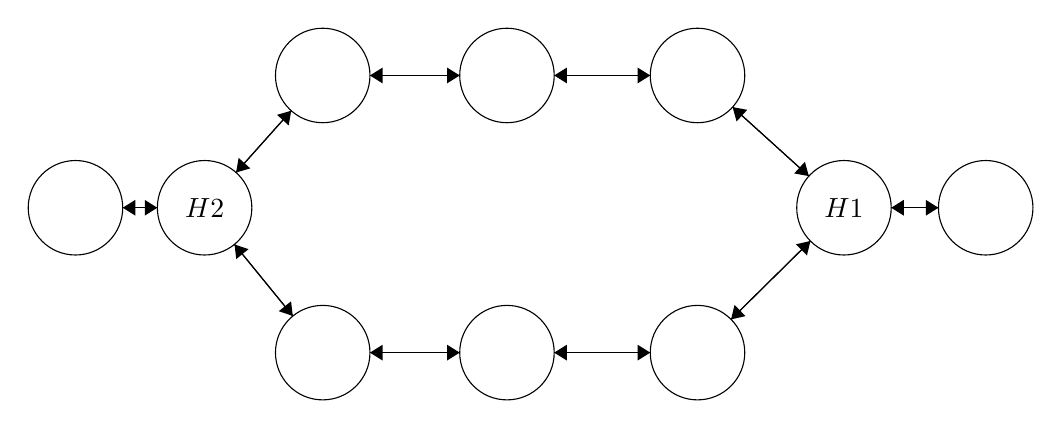
\begin{tikzpicture}[scale=0.2]
\tikzstyle{every node}+=[inner sep=0pt]
\draw [black] (17.9,-29.2) circle (3);
\draw (17.9,-29.2) node {$H2$};
\draw [black] (25.4,-20.8) circle (3);
\draw [black] (25.4,-38.4) circle (3);
\draw [black] (9.7,-29.2) circle (3);
\draw [black] (37.1,-38.4) circle (3);
\draw [black] (37.1,-20.8) circle (3);
\draw [black] (49.2,-38.4) circle (3);
\draw [black] (49.2,-20.8) circle (3);
\draw [black] (67.5,-29.2) circle (3);
\draw [black] (58.5,-29.2) circle (3);
\draw (58.5,-29.2) node {$H1$};
\draw [black] (51.33,-36.29) -- (56.37,-31.31);
\fill [black] (56.37,-31.31) -- (55.45,-31.52) -- (56.15,-32.23);
\draw [black] (51.43,-22.81) -- (56.27,-27.19);
\fill [black] (56.27,-27.19) -- (56.02,-26.28) -- (55.34,-27.02);
\draw [black] (61.5,-29.2) -- (64.5,-29.2);
\fill [black] (64.5,-29.2) -- (63.7,-28.7) -- (63.7,-29.7);
\draw [black] (64.5,-29.2) -- (61.5,-29.2);
\fill [black] (61.5,-29.2) -- (62.3,-29.7) -- (62.3,-28.7);
\draw [black] (56.27,-27.19) -- (51.43,-22.81);
\fill [black] (51.43,-22.81) -- (51.68,-23.72) -- (52.36,-22.98);
\draw [black] (56.37,-31.31) -- (51.33,-36.29);
\fill [black] (51.33,-36.29) -- (52.25,-36.08) -- (51.55,-35.37);
\draw [black] (40.1,-38.4) -- (46.2,-38.4);
\fill [black] (46.2,-38.4) -- (45.4,-37.9) -- (45.4,-38.9);
\draw [black] (46.2,-38.4) -- (40.1,-38.4);
\fill [black] (40.1,-38.4) -- (40.9,-38.9) -- (40.9,-37.9);
\draw [black] (46.2,-20.8) -- (40.1,-20.8);
\fill [black] (40.1,-20.8) -- (40.9,-21.3) -- (40.9,-20.3);
\draw [black] (40.1,-20.8) -- (46.2,-20.8);
\fill [black] (46.2,-20.8) -- (45.4,-20.3) -- (45.4,-21.3);
\draw [black] (28.4,-20.8) -- (34.1,-20.8);
\fill [black] (34.1,-20.8) -- (33.3,-20.3) -- (33.3,-21.3);
\draw [black] (34.1,-20.8) -- (28.4,-20.8);
\fill [black] (28.4,-20.8) -- (29.2,-21.3) -- (29.2,-20.3);
\draw [black] (28.4,-38.4) -- (34.1,-38.4);
\fill [black] (34.1,-38.4) -- (33.3,-37.9) -- (33.3,-38.9);
\draw [black] (34.1,-38.4) -- (28.4,-38.4);
\fill [black] (28.4,-38.4) -- (29.2,-38.9) -- (29.2,-37.9);
\draw [black] (19.8,-31.53) -- (23.5,-36.07);
\fill [black] (23.5,-36.07) -- (23.39,-35.14) -- (22.61,-35.77);
\draw [black] (23.5,-36.07) -- (19.8,-31.53);
\fill [black] (19.8,-31.53) -- (19.91,-32.46) -- (20.69,-31.83);
\draw [black] (23.4,-23.04) -- (19.9,-26.96);
\fill [black] (19.9,-26.96) -- (20.8,-26.7) -- (20.06,-26.03);
\draw [black] (19.9,-26.96) -- (23.4,-23.04);
\fill [black] (23.4,-23.04) -- (22.5,-23.3) -- (23.24,-23.97);
\draw [black] (14.9,-29.2) -- (12.7,-29.2);
\fill [black] (12.7,-29.2) -- (13.5,-29.7) -- (13.5,-28.7);
\draw [black] (12.7,-29.2) -- (14.9,-29.2);
\fill [black] (14.9,-29.2) -- (14.1,-28.7) -- (14.1,-29.7);
\end{tikzpicture}
\end{center}

\end{enumerate}

\end{document}